% Created by tikzDevice version 0.10.1 on 2016-09-01 14:54:32
% !TEX encoding = UTF-8 Unicode
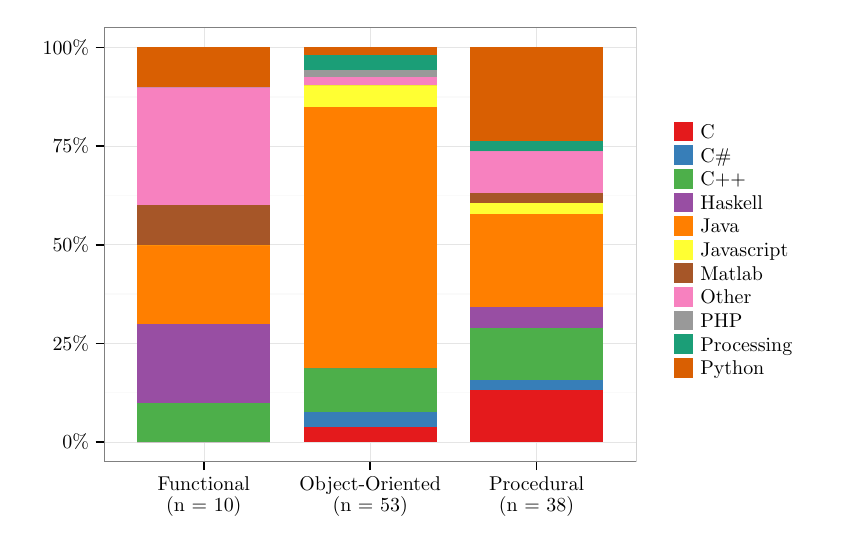
\begin{tikzpicture}[x=1pt,y=1pt]
\definecolor{fillColor}{RGB}{255,255,255}
\path[use as bounding box,fill=fillColor,fill opacity=0.00] (0,0) rectangle (289.08,180.67);
\begin{scope}
\path[clip] (  0.00,  0.00) rectangle (289.08,180.67);
\definecolor{drawColor}{RGB}{255,255,255}
\definecolor{fillColor}{RGB}{255,255,255}

\path[draw=drawColor,line width= 0.6pt,line join=round,line cap=round,fill=fillColor] (  0.00, -0.00) rectangle (289.08,180.67);
\end{scope}
\begin{scope}
\path[clip] ( 27.58, 23.83) rectangle (219.94,180.67);
\definecolor{fillColor}{RGB}{255,255,255}

\path[fill=fillColor] ( 27.58, 23.83) rectangle (219.94,180.67);
\definecolor{drawColor}{gray}{0.98}

\path[draw=drawColor,line width= 0.6pt,line join=round] ( 27.58, 48.78) --
	(219.94, 48.78);

\path[draw=drawColor,line width= 0.6pt,line join=round] ( 27.58, 84.43) --
	(219.94, 84.43);

\path[draw=drawColor,line width= 0.6pt,line join=round] ( 27.58,120.07) --
	(219.94,120.07);

\path[draw=drawColor,line width= 0.6pt,line join=round] ( 27.58,155.72) --
	(219.94,155.72);
\definecolor{drawColor}{gray}{0.90}

\path[draw=drawColor,line width= 0.2pt,line join=round] ( 27.58, 30.95) --
	(219.94, 30.95);

\path[draw=drawColor,line width= 0.2pt,line join=round] ( 27.58, 66.60) --
	(219.94, 66.60);

\path[draw=drawColor,line width= 0.2pt,line join=round] ( 27.58,102.25) --
	(219.94,102.25);

\path[draw=drawColor,line width= 0.2pt,line join=round] ( 27.58,137.90) --
	(219.94,137.90);

\path[draw=drawColor,line width= 0.2pt,line join=round] ( 27.58,173.55) --
	(219.94,173.55);

\path[draw=drawColor,line width= 0.2pt,line join=round] ( 63.65, 23.83) --
	( 63.65,180.67);

\path[draw=drawColor,line width= 0.2pt,line join=round] (123.76, 23.83) --
	(123.76,180.67);

\path[draw=drawColor,line width= 0.2pt,line join=round] (183.87, 23.83) --
	(183.87,180.67);
\definecolor{fillColor}{RGB}{228,26,28}

\path[fill=fillColor] ( 39.60, 30.95) rectangle ( 87.69, 30.95);
\definecolor{fillColor}{RGB}{55,126,184}

\path[fill=fillColor] ( 39.60, 30.95) rectangle ( 87.69, 30.95);
\definecolor{fillColor}{RGB}{77,175,74}

\path[fill=fillColor] ( 39.60, 30.95) rectangle ( 87.69, 45.21);
\definecolor{fillColor}{RGB}{152,78,163}

\path[fill=fillColor] ( 39.60, 45.21) rectangle ( 87.69, 73.73);
\definecolor{fillColor}{RGB}{255,127,0}

\path[fill=fillColor] ( 39.60, 73.73) rectangle ( 87.69,102.25);
\definecolor{fillColor}{RGB}{255,255,51}

\path[fill=fillColor] ( 39.60,102.25) rectangle ( 87.69,102.25);
\definecolor{fillColor}{RGB}{166,86,40}

\path[fill=fillColor] ( 39.60,102.25) rectangle ( 87.69,116.51);
\definecolor{fillColor}{RGB}{247,129,191}

\path[fill=fillColor] ( 39.60,116.51) rectangle ( 87.69,159.29);
\definecolor{fillColor}{gray}{0.60}

\path[fill=fillColor] ( 39.60,159.29) rectangle ( 87.69,159.29);
\definecolor{fillColor}{RGB}{27,158,119}

\path[fill=fillColor] ( 39.60,159.29) rectangle ( 87.69,159.29);
\definecolor{fillColor}{RGB}{217,95,2}

\path[fill=fillColor] ( 39.60,159.29) rectangle ( 87.69,173.55);
\definecolor{fillColor}{RGB}{228,26,28}

\path[fill=fillColor] ( 99.71, 30.95) rectangle (147.80, 36.34);
\definecolor{fillColor}{RGB}{55,126,184}

\path[fill=fillColor] ( 99.71, 36.34) rectangle (147.80, 41.72);
\definecolor{fillColor}{RGB}{77,175,74}

\path[fill=fillColor] ( 99.71, 41.72) rectangle (147.80, 57.86);
\definecolor{fillColor}{RGB}{152,78,163}

\path[fill=fillColor] ( 99.71, 57.86) rectangle (147.80, 57.86);
\definecolor{fillColor}{RGB}{255,127,0}

\path[fill=fillColor] ( 99.71, 57.86) rectangle (147.80,152.02);
\definecolor{fillColor}{RGB}{255,255,51}

\path[fill=fillColor] ( 99.71,152.02) rectangle (147.80,160.09);
\definecolor{fillColor}{RGB}{166,86,40}

\path[fill=fillColor] ( 99.71,160.09) rectangle (147.80,160.09);
\definecolor{fillColor}{RGB}{247,129,191}

\path[fill=fillColor] ( 99.71,160.09) rectangle (147.80,162.78);
\definecolor{fillColor}{gray}{0.60}

\path[fill=fillColor] ( 99.71,162.78) rectangle (147.80,165.47);
\definecolor{fillColor}{RGB}{27,158,119}

\path[fill=fillColor] ( 99.71,165.47) rectangle (147.80,170.86);
\definecolor{fillColor}{RGB}{217,95,2}

\path[fill=fillColor] ( 99.71,170.86) rectangle (147.80,173.55);
\definecolor{fillColor}{RGB}{228,26,28}

\path[fill=fillColor] (159.83, 30.95) rectangle (207.92, 49.72);
\definecolor{fillColor}{RGB}{55,126,184}

\path[fill=fillColor] (159.83, 49.72) rectangle (207.92, 53.47);
\definecolor{fillColor}{RGB}{77,175,74}

\path[fill=fillColor] (159.83, 53.47) rectangle (207.92, 72.23);
\definecolor{fillColor}{RGB}{152,78,163}

\path[fill=fillColor] (159.83, 72.23) rectangle (207.92, 79.74);
\definecolor{fillColor}{RGB}{255,127,0}

\path[fill=fillColor] (159.83, 79.74) rectangle (207.92,113.51);
\definecolor{fillColor}{RGB}{255,255,51}

\path[fill=fillColor] (159.83,113.51) rectangle (207.92,117.26);
\definecolor{fillColor}{RGB}{166,86,40}

\path[fill=fillColor] (159.83,117.26) rectangle (207.92,121.01);
\definecolor{fillColor}{RGB}{247,129,191}

\path[fill=fillColor] (159.83,121.01) rectangle (207.92,136.02);
\definecolor{fillColor}{gray}{0.60}

\path[fill=fillColor] (159.83,136.02) rectangle (207.92,136.02);
\definecolor{fillColor}{RGB}{27,158,119}

\path[fill=fillColor] (159.83,136.02) rectangle (207.92,139.77);
\definecolor{fillColor}{RGB}{217,95,2}

\path[fill=fillColor] (159.83,139.77) rectangle (207.92,173.55);
\definecolor{drawColor}{gray}{0.50}

\path[draw=drawColor,line width= 0.6pt,line join=round,line cap=round] ( 27.58, 23.83) rectangle (219.94,180.67);
\end{scope}
\begin{scope}
\path[clip] (  0.00,  0.00) rectangle (289.08,180.67);
\definecolor{drawColor}{RGB}{0,0,0}

\node[text=drawColor,anchor=base east,inner sep=0pt, outer sep=0pt, scale=  0.72] at ( 22.18, 28.48) {0\%};

\node[text=drawColor,anchor=base east,inner sep=0pt, outer sep=0pt, scale=  0.72] at ( 22.18, 64.12) {25\%};

\node[text=drawColor,anchor=base east,inner sep=0pt, outer sep=0pt, scale=  0.72] at ( 22.18, 99.77) {50\%};

\node[text=drawColor,anchor=base east,inner sep=0pt, outer sep=0pt, scale=  0.72] at ( 22.18,135.42) {75\%};

\node[text=drawColor,anchor=base east,inner sep=0pt, outer sep=0pt, scale=  0.72] at ( 22.18,171.07) {100\%};
\end{scope}
\begin{scope}
\path[clip] (  0.00,  0.00) rectangle (289.08,180.67);
\definecolor{drawColor}{RGB}{0,0,0}

\path[draw=drawColor,line width= 0.6pt,line join=round] ( 24.58, 30.95) --
	( 27.58, 30.95);

\path[draw=drawColor,line width= 0.6pt,line join=round] ( 24.58, 66.60) --
	( 27.58, 66.60);

\path[draw=drawColor,line width= 0.6pt,line join=round] ( 24.58,102.25) --
	( 27.58,102.25);

\path[draw=drawColor,line width= 0.6pt,line join=round] ( 24.58,137.90) --
	( 27.58,137.90);

\path[draw=drawColor,line width= 0.6pt,line join=round] ( 24.58,173.55) --
	( 27.58,173.55);
\end{scope}
\begin{scope}
\path[clip] (  0.00,  0.00) rectangle (289.08,180.67);
\definecolor{drawColor}{RGB}{0,0,0}

\path[draw=drawColor,line width= 0.6pt,line join=round] ( 63.65, 20.83) --
	( 63.65, 23.83);

\path[draw=drawColor,line width= 0.6pt,line join=round] (123.76, 20.83) --
	(123.76, 23.83);

\path[draw=drawColor,line width= 0.6pt,line join=round] (183.87, 20.83) --
	(183.87, 23.83);
\end{scope}
\begin{scope}
\path[clip] (  0.00,  0.00) rectangle (289.08,180.67);
\definecolor{drawColor}{RGB}{0,0,0}

\node[text=drawColor,anchor=base,inner sep=0pt, outer sep=0pt, scale=  0.72] at ( 63.65, 13.47) {Functional};

\node[text=drawColor,anchor=base,inner sep=0pt, outer sep=0pt, scale=  0.72] at ( 63.65,  5.69) {(n = 10)};

\node[text=drawColor,anchor=base,inner sep=0pt, outer sep=0pt, scale=  0.72] at (123.76, 13.47) {Object-Oriented};

\node[text=drawColor,anchor=base,inner sep=0pt, outer sep=0pt, scale=  0.72] at (123.76,  5.69) {(n = 53)};

\node[text=drawColor,anchor=base,inner sep=0pt, outer sep=0pt, scale=  0.72] at (183.87, 13.47) {Procedural};

\node[text=drawColor,anchor=base,inner sep=0pt, outer sep=0pt, scale=  0.72] at (183.87,  5.69) {(n = 38)};
\end{scope}
\begin{scope}
\path[clip] (  0.00,  0.00) rectangle (289.08,180.67);
\definecolor{fillColor}{RGB}{255,255,255}

\path[fill=fillColor] (228.47, 49.23) rectangle (280.54,155.27);
\end{scope}
\begin{scope}
\path[clip] (  0.00,  0.00) rectangle (289.08,180.67);
\definecolor{fillColor}{RGB}{228,26,28}

\path[fill=fillColor] (233.45,139.57) rectangle (240.57,146.68);
\end{scope}
\begin{scope}
\path[clip] (  0.00,  0.00) rectangle (289.08,180.67);
\definecolor{fillColor}{RGB}{55,126,184}

\path[fill=fillColor] (233.45,131.03) rectangle (240.57,138.14);
\end{scope}
\begin{scope}
\path[clip] (  0.00,  0.00) rectangle (289.08,180.67);
\definecolor{fillColor}{RGB}{77,175,74}

\path[fill=fillColor] (233.45,122.49) rectangle (240.57,129.61);
\end{scope}
\begin{scope}
\path[clip] (  0.00,  0.00) rectangle (289.08,180.67);
\definecolor{fillColor}{RGB}{152,78,163}

\path[fill=fillColor] (233.45,113.96) rectangle (240.57,121.07);
\end{scope}
\begin{scope}
\path[clip] (  0.00,  0.00) rectangle (289.08,180.67);
\definecolor{fillColor}{RGB}{255,127,0}

\path[fill=fillColor] (233.45,105.42) rectangle (240.57,112.54);
\end{scope}
\begin{scope}
\path[clip] (  0.00,  0.00) rectangle (289.08,180.67);
\definecolor{fillColor}{RGB}{255,255,51}

\path[fill=fillColor] (233.45, 96.89) rectangle (240.57,104.00);
\end{scope}
\begin{scope}
\path[clip] (  0.00,  0.00) rectangle (289.08,180.67);
\definecolor{fillColor}{RGB}{166,86,40}

\path[fill=fillColor] (233.45, 88.35) rectangle (240.57, 95.46);
\end{scope}
\begin{scope}
\path[clip] (  0.00,  0.00) rectangle (289.08,180.67);
\definecolor{fillColor}{RGB}{247,129,191}

\path[fill=fillColor] (233.45, 79.82) rectangle (240.57, 86.93);
\end{scope}
\begin{scope}
\path[clip] (  0.00,  0.00) rectangle (289.08,180.67);
\definecolor{fillColor}{gray}{0.60}

\path[fill=fillColor] (233.45, 71.28) rectangle (240.57, 78.39);
\end{scope}
\begin{scope}
\path[clip] (  0.00,  0.00) rectangle (289.08,180.67);
\definecolor{fillColor}{RGB}{27,158,119}

\path[fill=fillColor] (233.45, 62.74) rectangle (240.57, 69.86);
\end{scope}
\begin{scope}
\path[clip] (  0.00,  0.00) rectangle (289.08,180.67);
\definecolor{fillColor}{RGB}{217,95,2}

\path[fill=fillColor] (233.45, 54.21) rectangle (240.57, 61.32);
\end{scope}
\begin{scope}
\path[clip] (  0.00,  0.00) rectangle (289.08,180.67);
\definecolor{drawColor}{RGB}{0,0,0}

\node[text=drawColor,anchor=base west,inner sep=0pt, outer sep=0pt, scale=  0.72] at (243.08,140.64) {C};
\end{scope}
\begin{scope}
\path[clip] (  0.00,  0.00) rectangle (289.08,180.67);
\definecolor{drawColor}{RGB}{0,0,0}

\node[text=drawColor,anchor=base west,inner sep=0pt, outer sep=0pt, scale=  0.72] at (243.08,132.11) {C\#};
\end{scope}
\begin{scope}
\path[clip] (  0.00,  0.00) rectangle (289.08,180.67);
\definecolor{drawColor}{RGB}{0,0,0}

\node[text=drawColor,anchor=base west,inner sep=0pt, outer sep=0pt, scale=  0.72] at (243.08,123.57) {C++};
\end{scope}
\begin{scope}
\path[clip] (  0.00,  0.00) rectangle (289.08,180.67);
\definecolor{drawColor}{RGB}{0,0,0}

\node[text=drawColor,anchor=base west,inner sep=0pt, outer sep=0pt, scale=  0.72] at (243.08,115.04) {Haskell};
\end{scope}
\begin{scope}
\path[clip] (  0.00,  0.00) rectangle (289.08,180.67);
\definecolor{drawColor}{RGB}{0,0,0}

\node[text=drawColor,anchor=base west,inner sep=0pt, outer sep=0pt, scale=  0.72] at (243.08,106.50) {Java};
\end{scope}
\begin{scope}
\path[clip] (  0.00,  0.00) rectangle (289.08,180.67);
\definecolor{drawColor}{RGB}{0,0,0}

\node[text=drawColor,anchor=base west,inner sep=0pt, outer sep=0pt, scale=  0.72] at (243.08, 97.96) {Javascript};
\end{scope}
\begin{scope}
\path[clip] (  0.00,  0.00) rectangle (289.08,180.67);
\definecolor{drawColor}{RGB}{0,0,0}

\node[text=drawColor,anchor=base west,inner sep=0pt, outer sep=0pt, scale=  0.72] at (243.08, 89.43) {Matlab};
\end{scope}
\begin{scope}
\path[clip] (  0.00,  0.00) rectangle (289.08,180.67);
\definecolor{drawColor}{RGB}{0,0,0}

\node[text=drawColor,anchor=base west,inner sep=0pt, outer sep=0pt, scale=  0.72] at (243.08, 80.89) {Other};
\end{scope}
\begin{scope}
\path[clip] (  0.00,  0.00) rectangle (289.08,180.67);
\definecolor{drawColor}{RGB}{0,0,0}

\node[text=drawColor,anchor=base west,inner sep=0pt, outer sep=0pt, scale=  0.72] at (243.08, 72.36) {PHP};
\end{scope}
\begin{scope}
\path[clip] (  0.00,  0.00) rectangle (289.08,180.67);
\definecolor{drawColor}{RGB}{0,0,0}

\node[text=drawColor,anchor=base west,inner sep=0pt, outer sep=0pt, scale=  0.72] at (243.08, 63.82) {Processing};
\end{scope}
\begin{scope}
\path[clip] (  0.00,  0.00) rectangle (289.08,180.67);
\definecolor{drawColor}{RGB}{0,0,0}

\node[text=drawColor,anchor=base west,inner sep=0pt, outer sep=0pt, scale=  0.72] at (243.08, 55.28) {Python};
\end{scope}
\end{tikzpicture}
